\section{گام تکمیلی: ارزیابی شبکه‌ی اختصاصی \lr{(Scratch)} و مقایسه جامع}

به منظور تکمیل الزامات پروژه و ایجاد یک بستر مقایسه‌ی کاملاً عادلانه بین یادگیری انتقالی و یادگیری از پایه \lr{(Training from Scratch)}، معماری \lr{Custom CNN} که پیش‌تر طراحی شده بود، با همان شرایط دقیقاً به مدت ۳۰ دوره آموزش دید.

\subsection{تحلیل همگرایی و رفتار تابع زیان شبکه‌ی اختصاصی}
فرآیند آموزش این شبکه حدود ۶۶ دقیقه زمان برد (میانگین \lr{132} ثانیه برای هر دوره). نمودارهای آموزش در شکل \ref{fig:custom_curves} رسم شده‌اند.

\begin{figure}[h!]
    \centering
    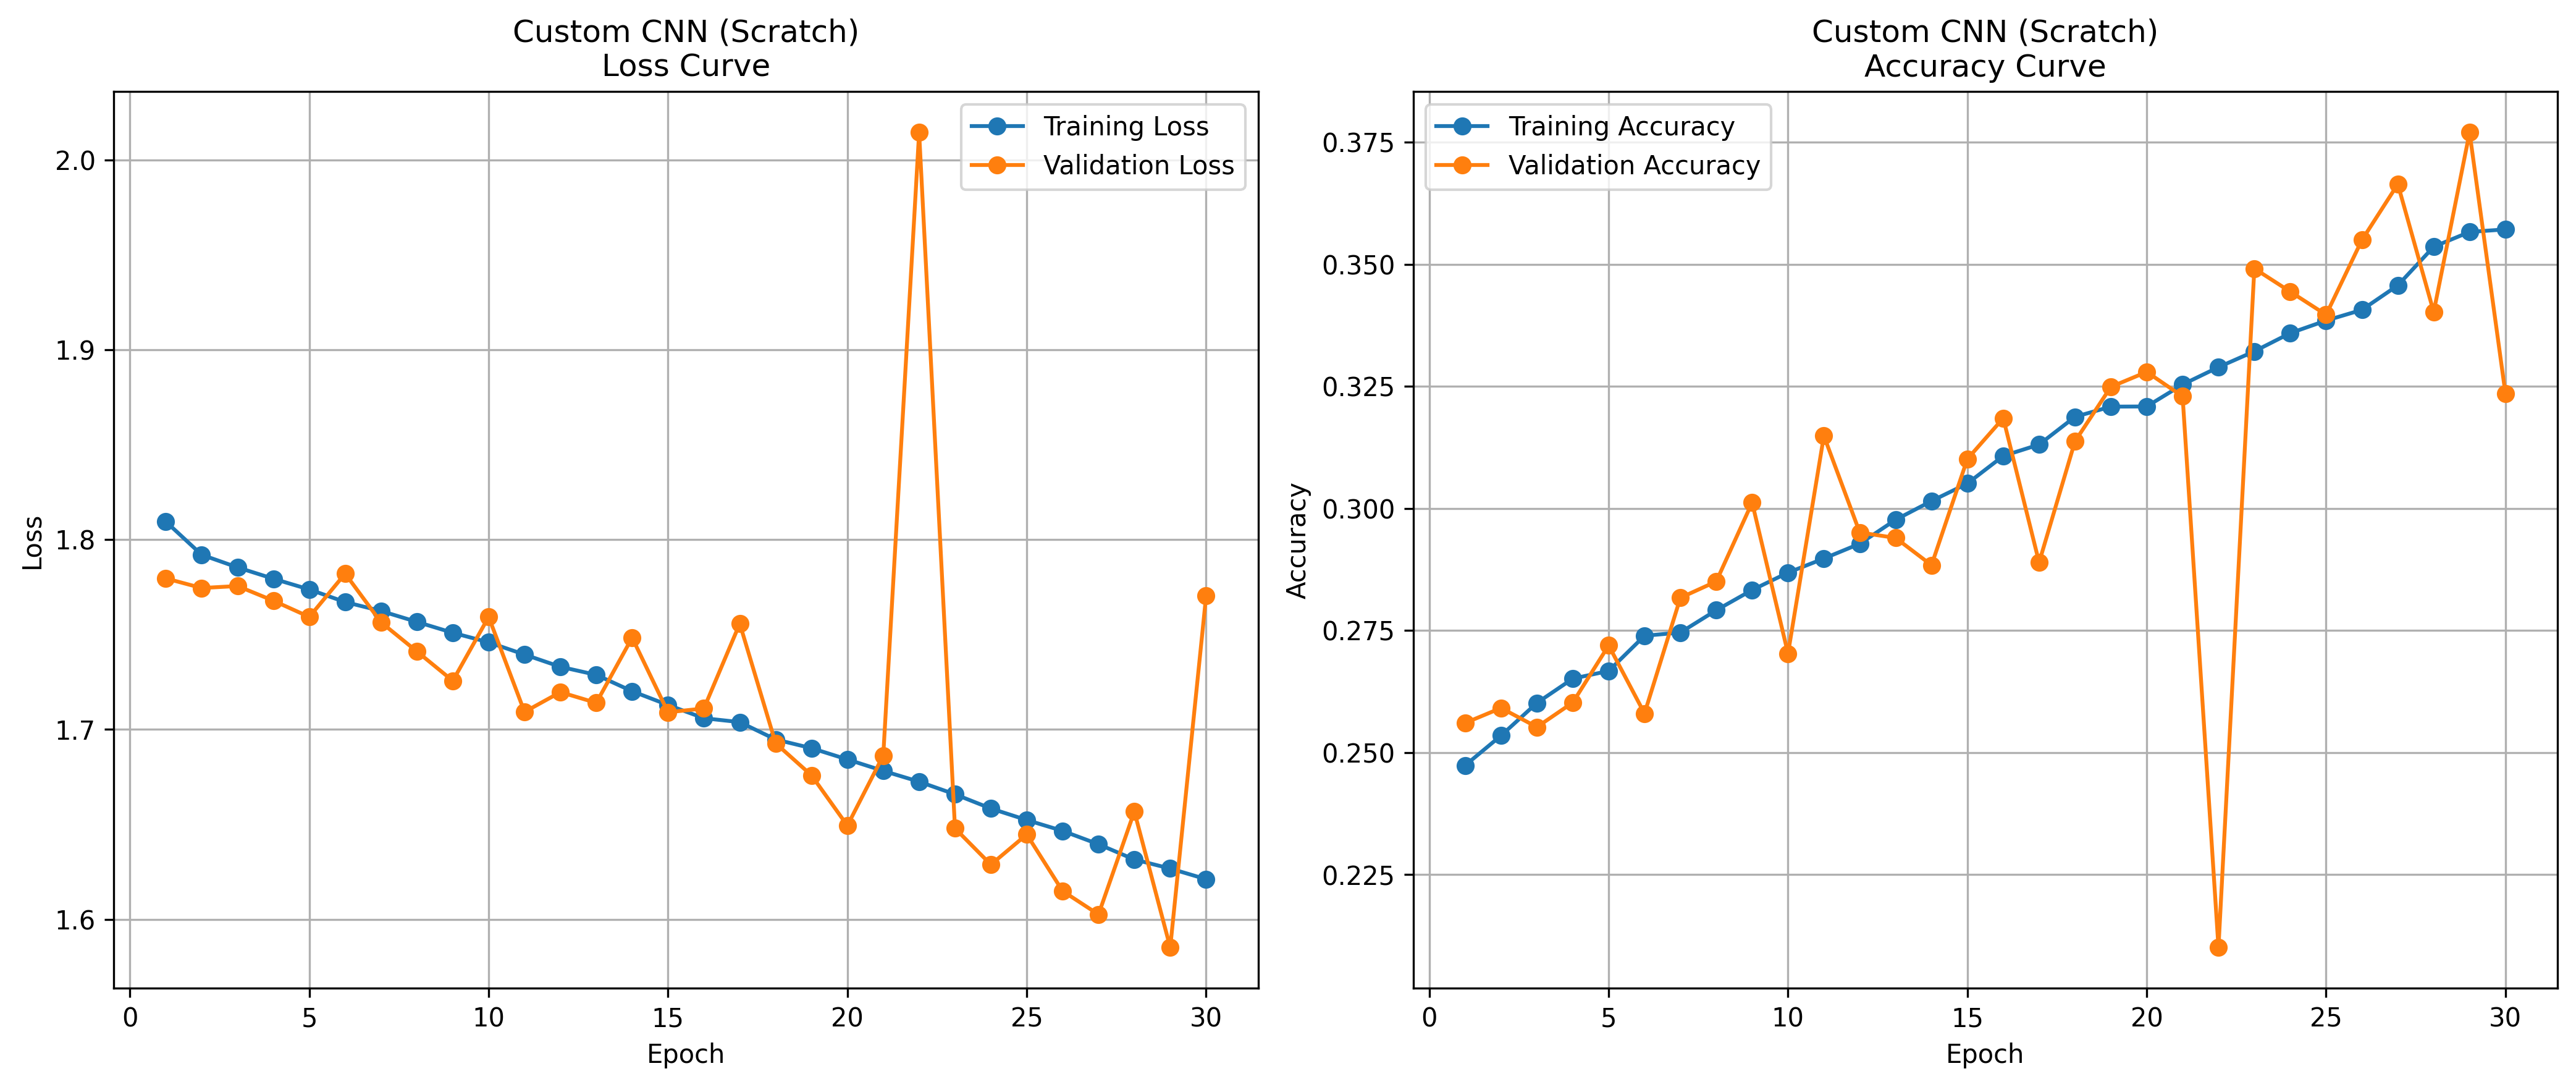
\includegraphics[width=1\textwidth]{images/custom_cnn_curves.png}
    \caption{منحنی‌های خطا و دقت شبکه‌ی \lr{Custom CNN} (آموزش با وزن‌های تصادفی)}
    \label{fig:custom_curves}
\end{figure}

برخلاف مدل‌های یادگیری انتقالی، رفتار تابع زیان اعتبارسنجی \lr{(Validation Loss)} در این شبکه به شدت ناپایدار است (به‌ویژه پرش‌های شدید در دوره‌های ۲۲ و ۳۰). این نوسانات نشان می‌دهد که شبکه به دلیل شروع با وزن‌های کاملاً تصادفی و پیچیدگی بالای دیتاست \lr{FER2013}، در یافتن یک کمینه‌ی عمومی پایدار \lr{(Global Minimum)} دچار مشکل است. بهترین دقت اعتبارسنجی در دوره‌ی ۲۹ و معادل \lr{37.70\%} ثبت شد.

\subsection{ارزیابی نهایی و تحلیل ماتریس درهم‌ریختگی}
پس از ارزیابی مدل روی مجموعه‌ی آزمون، دقت نهایی \lr{38\%} به دست آمد. گزارش دسته‌بندی و ماتریس درهم‌ریختگی (شکل \ref{fig:custom_cm}) حقایق مهمی را روشن می‌کنند:

\begin{itemize}
    \item \textbf{فروپاشی در کلاس‌های اقلیت:} شبکه در تشخیص احساسات خشم \lr{(Angry)} و انزجار \lr{(Disgust)} کاملاً شکست خورده است (\lr{Recall} برابر با صفر).
    \item \textbf{سوگیری شدید \lr{(Bias)}:} مدل به شدت به سمت پیش‌بینی کلاس اکثریت یعنی شادی \lr{(Happy)} با ۷۰۰ پیش‌بینی متمایل شده است که نشان از عدم توانایی شبکه‌ی کوچک در استخراج ویژگی‌های متمایزکننده دارد.
\end{itemize}

\begin{figure}[h!]
    \centering
    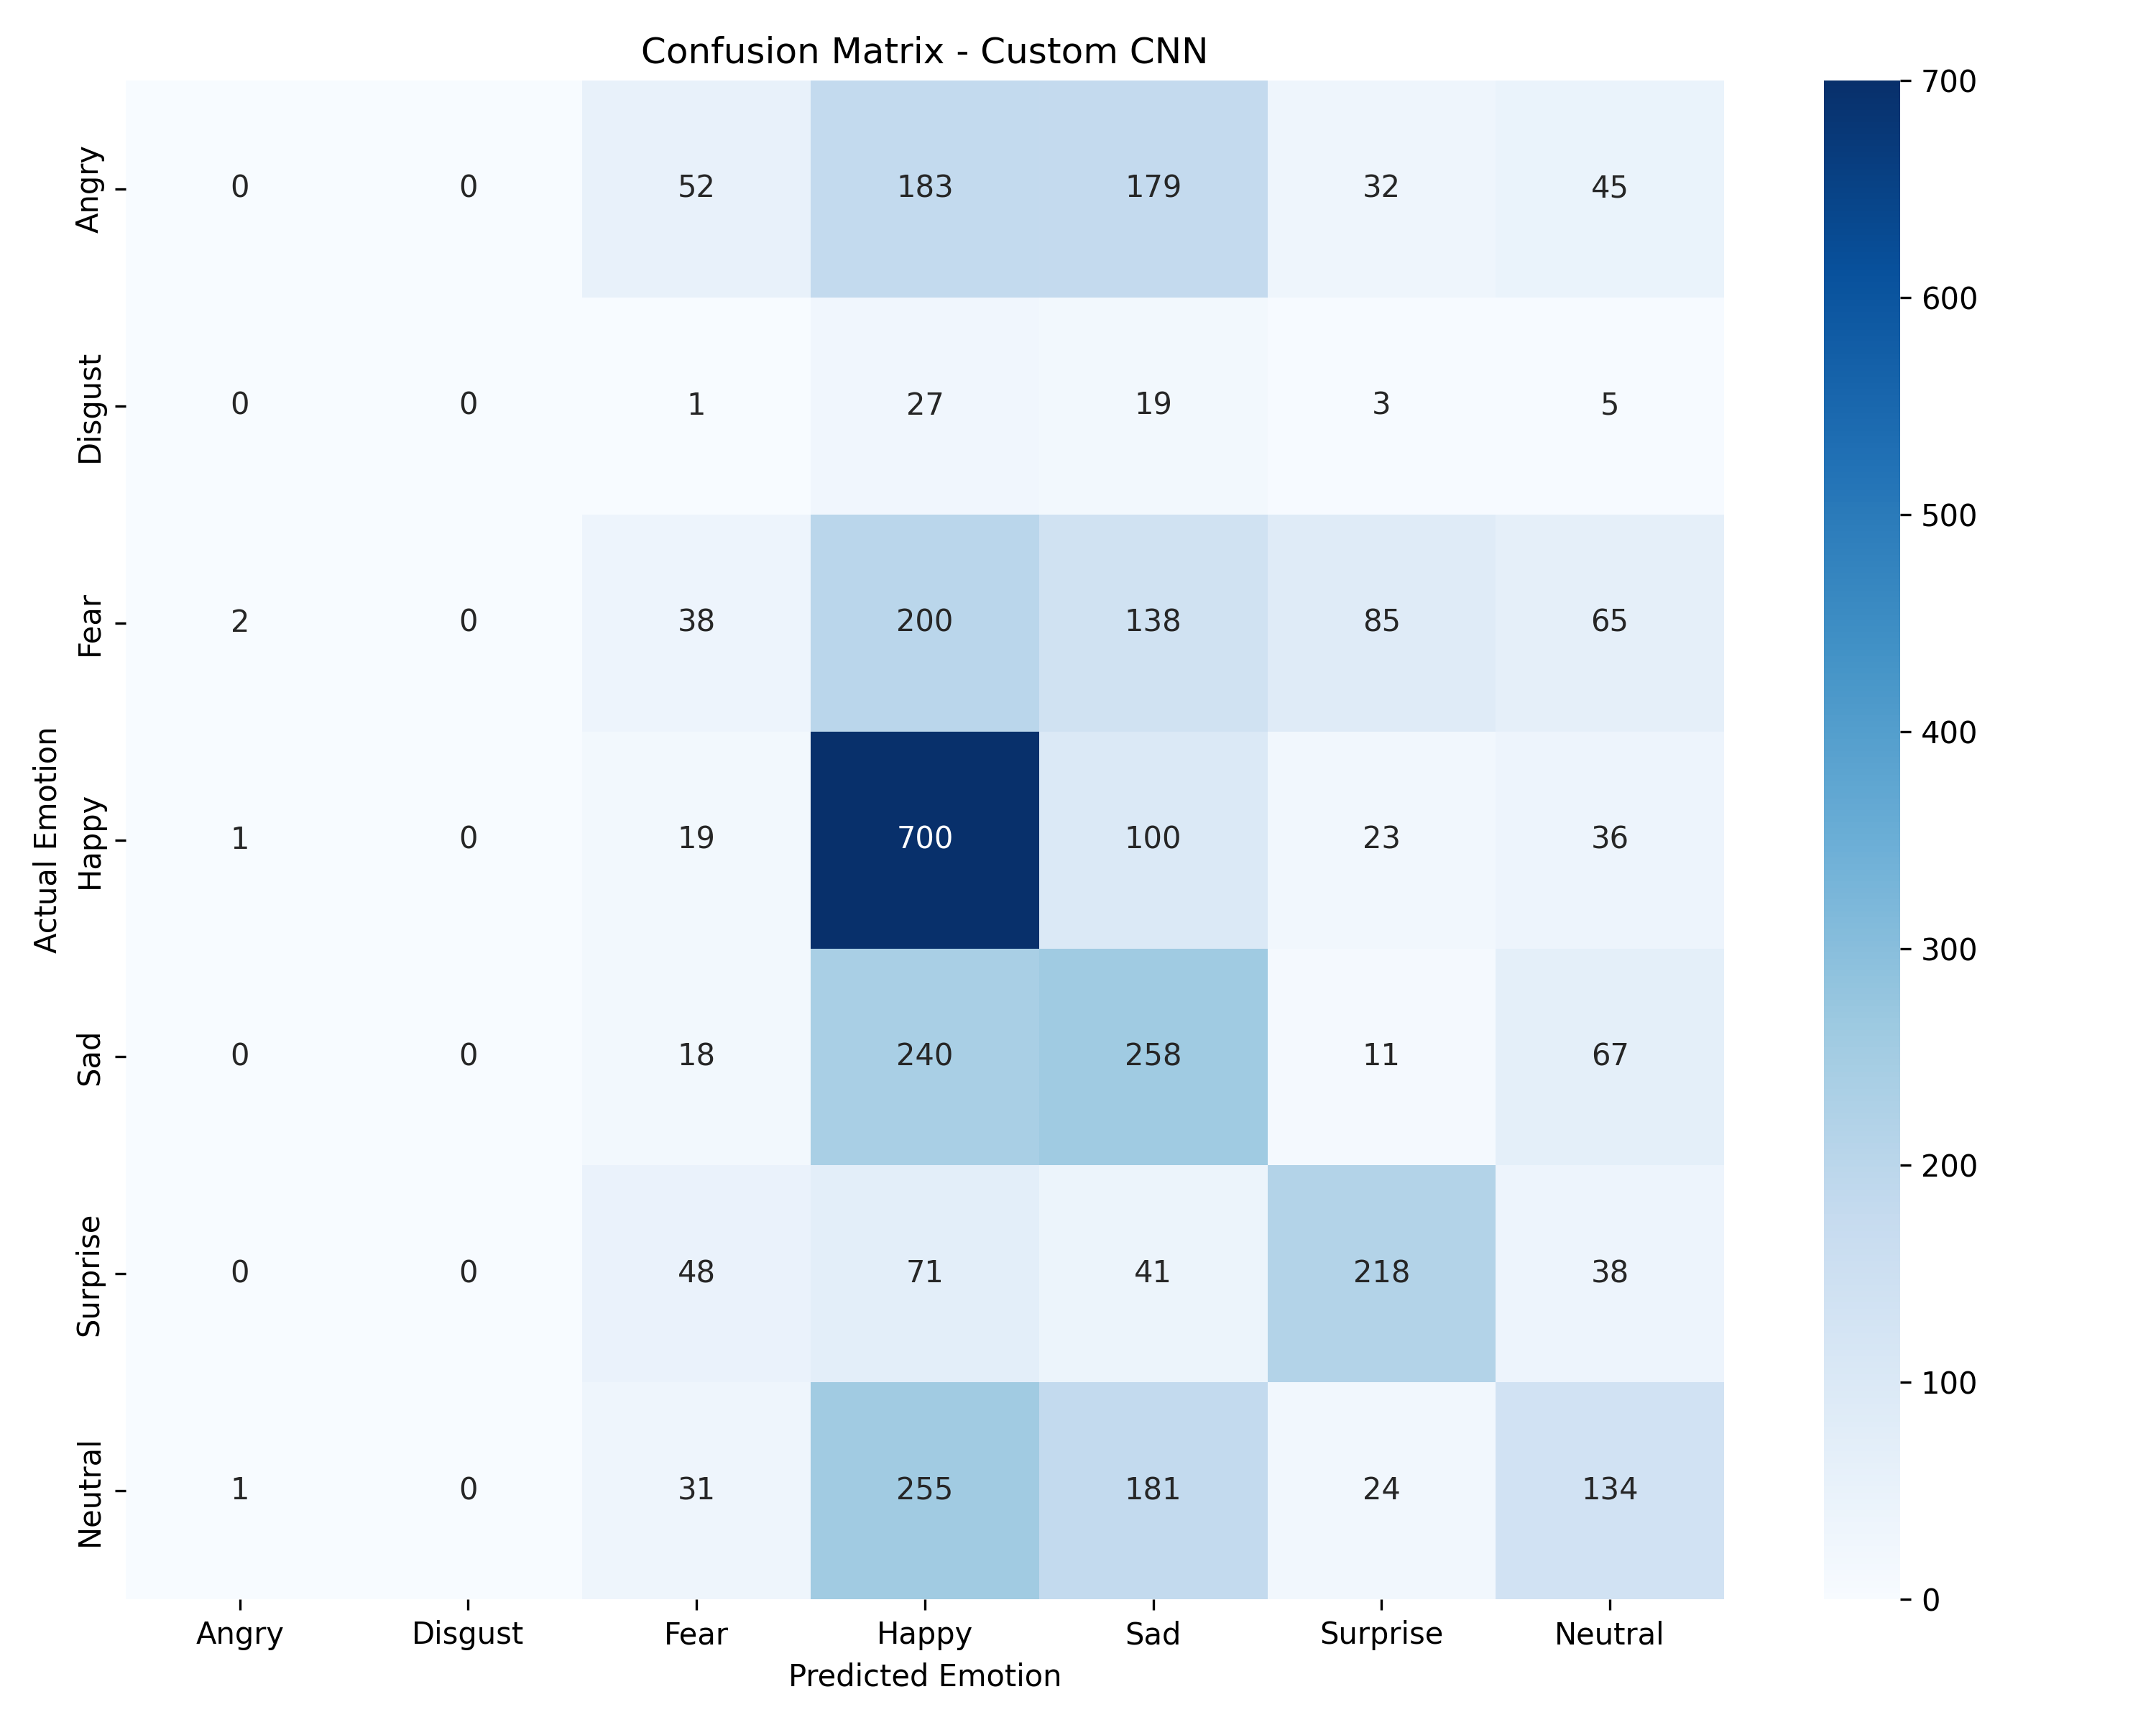
\includegraphics[width=0.85\textwidth]{images/custom_cnn_cm.png}
    \caption{ماتریس درهم‌ریختگی مدل \lr{Custom CNN} روی داده‌های آزمون}
    \label{fig:custom_cm}
\end{figure}

\subsection{مقایسه‌ی نهایی: یادگیری انتقالی در برابر آموزش از پایه}
با کنار هم قرار دادن نتایج این سه مدل، تحلیل‌های زیر استنتاج می‌گردد:

\begin{enumerate}
    \item \textbf{تفاوت خیره‌کننده در عملکرد:} مدل \lr{Fine-Tuned ResNet18} با رسیدن به دقت \lr{66\%} توانست مدل \lr{Custom CNN} (با دقت \lr{38\%}) را با اختلاف فاحش \lr{28} درصد شکست دهد. وزن‌های از پیش آموزش‌دیده‌ی \lr{ImageNet} نقش یک کاتالیزور قدرتمند را برای درک اولیه‌ی لبه‌ها و بافت‌ها ایفا کردند.
    \item \textbf{گلوگاه محاسباتی \lr{(Computational Bottleneck)}:} میانگین زمان آموزش هر دوره برای شبکه‌ی \lr{Custom CNN} با تنها ۱۰۰ هزار پارامتر، \lr{132} ثانیه بود؛ در حالی که این زمان برای \lr{ResNet18} با ۱۱ میلیون پارامتر، \lr{126} ثانیه ثبت شد! این مشاهده‌ی مهم ثابت می‌کند که در سیستم فعلی، گلوگاه اصلی مربوط به پردازش ماتریس‌ها در \lr{GPU} نیست، بلکه مربوط به عملیات \lr{I/O} (خواندن تصاویر از دیسک) و پیش‌پردازش‌های \lr{CPU-bound} در \lr{DataLoader} است.
    \item \textbf{تأثیر تعداد پارامتر بر تعمیم‌پذیری:} شبکه‌ی \lr{Custom CNN} به دلیل ظرفیت پایین (تعداد کم پارامترها و لایه‌ها)، حتی با وجود تکنیک‌های منظم‌سازی \lr{(Regularization)} نتوانست الگوهای پیچیده‌ی چهره را کشف کند. در مقابل، معماری عمیق \lr{ResNet} با اتصالات میان‌بر \lr{(Skip Connections)}، توانایی بسیار بالاتری در تعمیم‌پذیری و کنترل مشکل محوشدگی گرادیان \lr{(Vanishing Gradient)} از خود نشان داد.
\end{enumerate}